\chapter{SmartEduTrack: Hệ thống theo dõi học tập thông minh hỗ trợ ra quyết định quản lý}
\label{chap:chap6}
\section{Giới thiệu SmartEduTrack}
SmartEduTrack là một nền tảng website giúp người quản lý khóa học giám sát học viên. Xuất phát từ một dự án nghiên cứu về ứng dụng Deep Learning trong giáo dục, chúng tôi đã phát triển SmartEduTrack nhằm hiện thực hóa tiềm năng của AI trong giáo dục trực tuyến.

Website có các chức năng giúp theo dõi hiệu suất học viên, giúp người quản lý có được những kế hoạch và giải pháp kịp thời. Điểm đặc biệt của SmartEduTrack là việc tích hợp một mô hình có thể dự đoán khả năng hoàn thành khóa học của từng học viên chỉ trong 3 tuần đầu kể từ khi người học bắt đầu. Điều này giúp các nhà quản lý phát hiện kịp thời những học viên có nguy cơ gặp khó khăn hoặc bỏ học, từ đó cung cấp sự hỗ trợ cá nhân hóa và can thiệp sớm, tối ưu hóa cơ hội thành công cho tất cả người học.
\section{Phân tích thiết kế}
 \textbf{SmartEduTrack} được phân tích thiết kế để đáp ứng các mục tiêu chính bao gồm:

\begin{itemize}
    \item Đưa ra dự đoán chuẩn xác về kết quả học tập của người học ngay trong những tuần đầu của khóa học.
    \item Cung cấp giao diện trực quan, thân thiện với các chức năng hữu ích nhằm hỗ trợ tối đa cho người quản lý khóa học.

\end{itemize}

SmartEduTrack được thiết kế với các chức năng cốt lõi tập trung phục vụ một nhóm người dùng duy nhất, đó là \textbf{người quản lý khóa học}.

\begin{table}[H]
\centering
\caption{Bảng Use Case của hệ thống SmartEduTrack}
\label{tab:usecase}
\renewcommand{\arraystretch}{1.2} % tăng độ cao dòng
\begin{tabular}{|c|p{5cm}|p{3cm}|p{4.5cm}|}
\hline
\multicolumn{1}{|c|}{\textbf{STT}} & \multicolumn{1}{c|}{\textbf{Use Case}} & \multicolumn{1}{c|}{\textbf{Tác nhân}} & \multicolumn{1}{c|}{\textbf{Trang}} \\
\hline
1 & Xem danh sách người học & Course assistant & Education Management \\
\hline
2 & Bộ lọc người học theo khóa học hoặc tháng/năm đăng ký khóa học & Course assistant & Education Management \\
\hline
3 & Xem chi tiết hành vi người học & Course assistant & Education Management \\
\hline
4 & Xem xu hướng học tập của người học & Course assistant & Education Management \\
\hline
5 & Dự đoán kết quả hoàn thành khóa học & Course assistant & Education Management \\
\hline
6 & Xuất report & Course assistant & Education Management \\
\hline
7 & Xem danh sách 5 khóa học ghi nhận số người học bỏ dở nhiều nhất & Course assistant & Education Management \\
\hline
8 & Xem tổng quát bộ dữ liệu MOOCs & Course assistant & Overview \\
\hline
9 & Xem chi tiết từng file dữ liệu MOOCs & Course assistant & Overview \\
\hline
10 & Xem tỷ lệ khuyết của từng file dữ liệu & Course assistant & Overview \\
\hline
11 & Xem chi tiết mô tả bộ dữ liệu hành vi người học & Course assistant & Data Quality \\
\hline
12 & Xem số lượng và tỉ lệ nhãn được dự đoán cho từng người học & Course assistant & Data Quality \\
\hline
13 & Xem chất lượng dữ liệu theo độ đo completeness và consisitency & Course assistant & Data Quality \\
\hline
14 & Bộ lọc xem hiệu suất dự đoán của từng mô hình & Course assistant & Data Quality \\
\hline
\end{tabular}
\end{table}


\section{Kiến trúc hệ thống}
% Front-end, Backend: Sử dụng ngôn ngữ gì, có chức năng gì, sử dụng database gì
\begin{figure}[H]
    \centering
    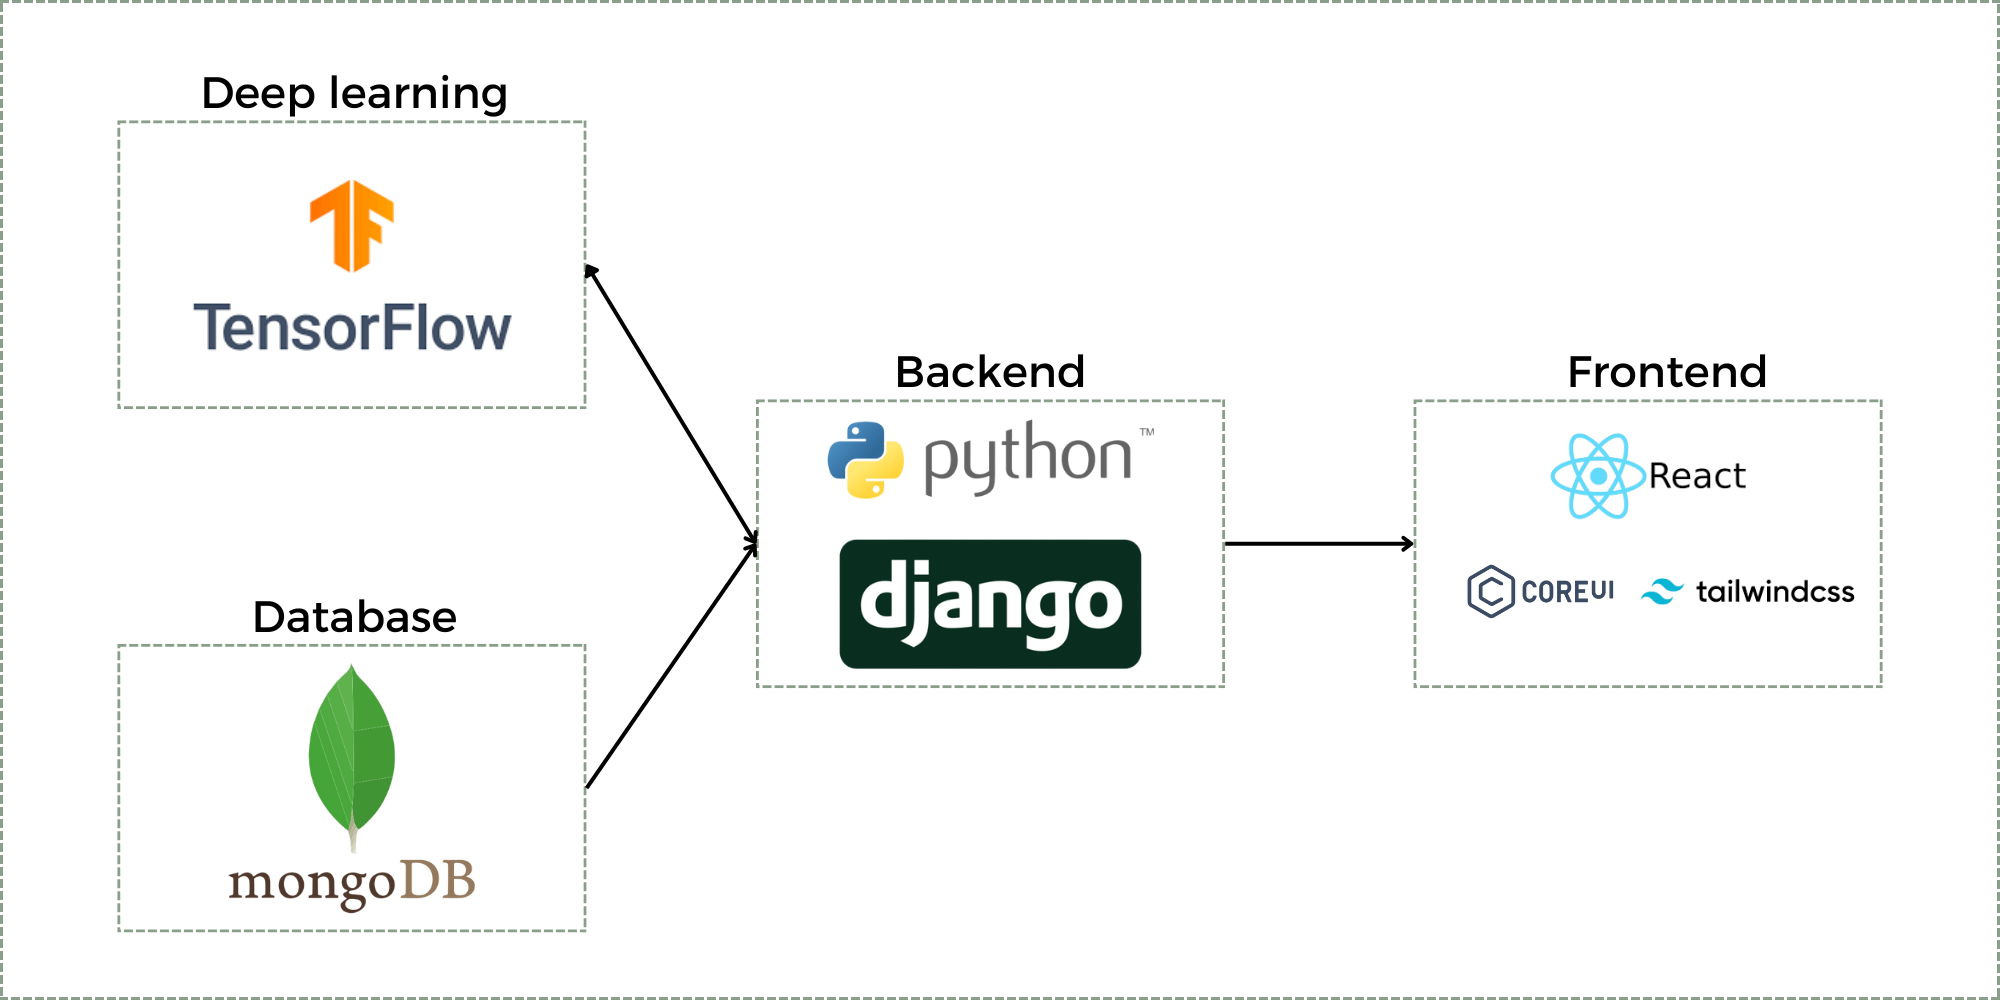
\includegraphics[width = 0.8\textwidth]{imgs/website-system-architecture.png}
    \caption{Kiến trúc hệ thống website SmartEduTrack}
    \label{fig:website-system-architecture}
\end{figure}
SmartEduTrack phát triển dựa trên cấu trúc \textbf{Client-Server}. Mỗi lớp có một nhiệm vụ chuyên biệt và tương tác với nhau qua các giao diện được định nghĩa rõ ràng:

\begin{itemize}
    \item \textbf{Lớp giao diện người dùng (Frontend):} Xây dựng bằng \textit{ReactJS} và \textit{TailwindCSS} để tạo ra một giao diện trực quan, đáp ứng nhanh và thân thiện.
    
    \item \textbf{Lớp xử lý nghiệp vụ (Backend):} Nền tảng Python được sử dụng thông qua framework Django. Nhiệm vụ chính của nó bao gồm xử lý các yêu cầu từ phía giao diện, trao đổi thông tin với database và tích hợp mô hình học sâu để thực hiện dự đoán kết quả hoàn thành khóa học.
    
    \item \textbf{Lớp dữ liệu (Database):} Lớp này sử dụng \textit{MongoDB} làm hệ quản trị cơ sở dữ liệu NoSQL, có nhiệm vụ lưu trữ và quản lý toàn bộ dữ liệu của hệ thống. Dữ liệu này bao gồm hồ sơ chi tiết của học viên, dữ liệu quá trình tương tác học tập, và các kết quả dự đoán được tạo ra bởi mô hình.
\end{itemize}

\section{SmartEduTrack - Demo}
% chụp hình giới thiệu trang web
\subsection{Chức năng: Xem danh sách người học}
\begin{figure}[H]
    \centering
    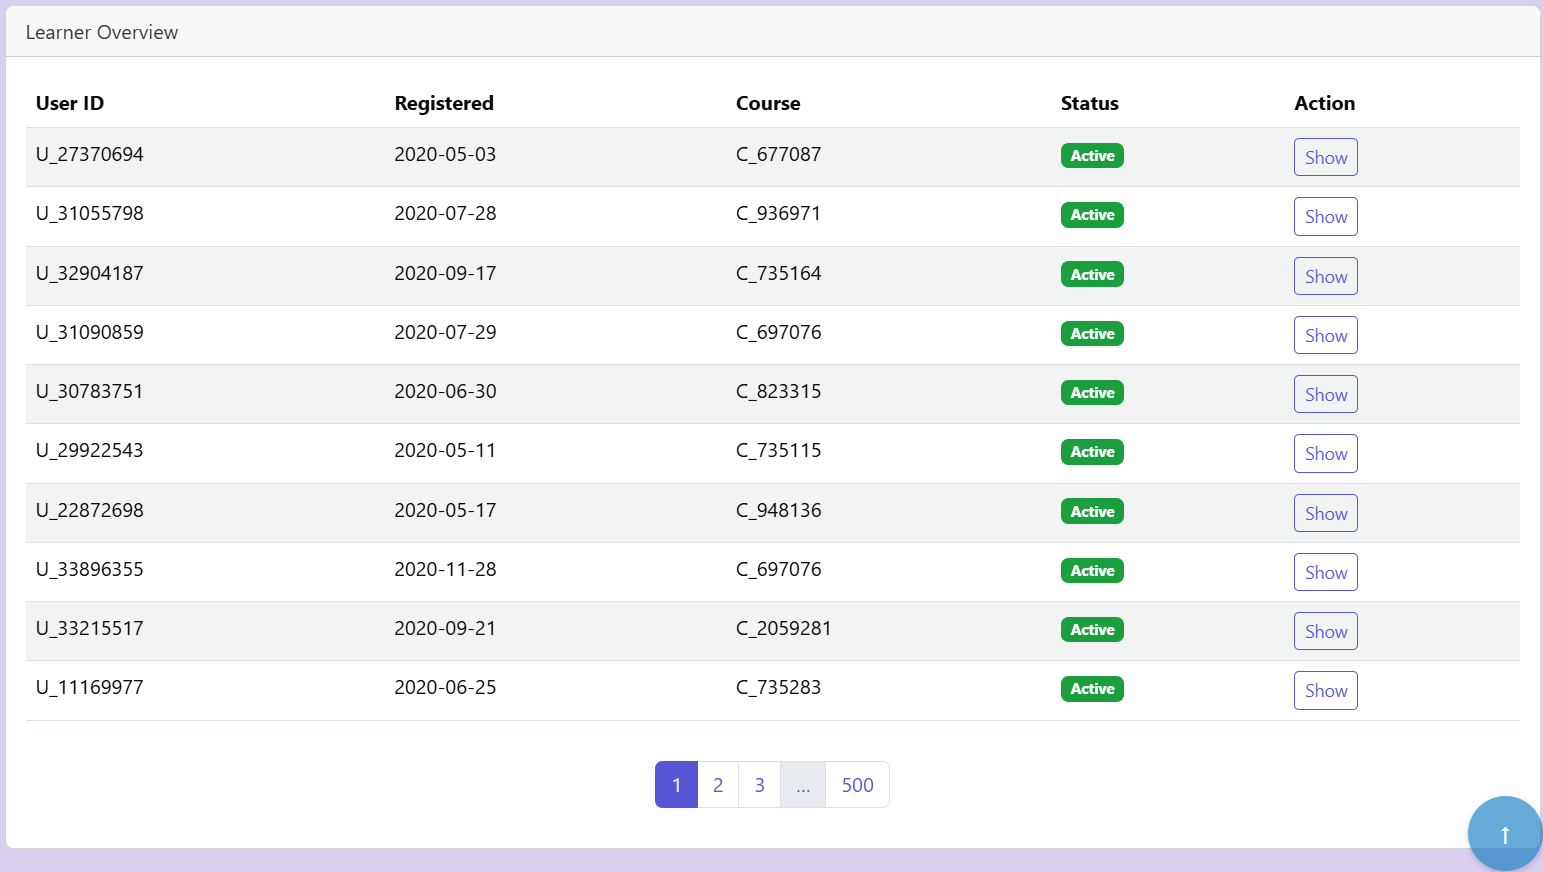
\includegraphics[width = 0.8\textwidth]{imgs/demo-1.png}
    \caption{Danh sách người học}
    \label{fig:demo-1}
\end{figure}
\subsection{Chức năng: Lọc người học theo khóa học hoặc tháng/năm đăng ký khóa học}
\begin{figure}[H]
    \centering
    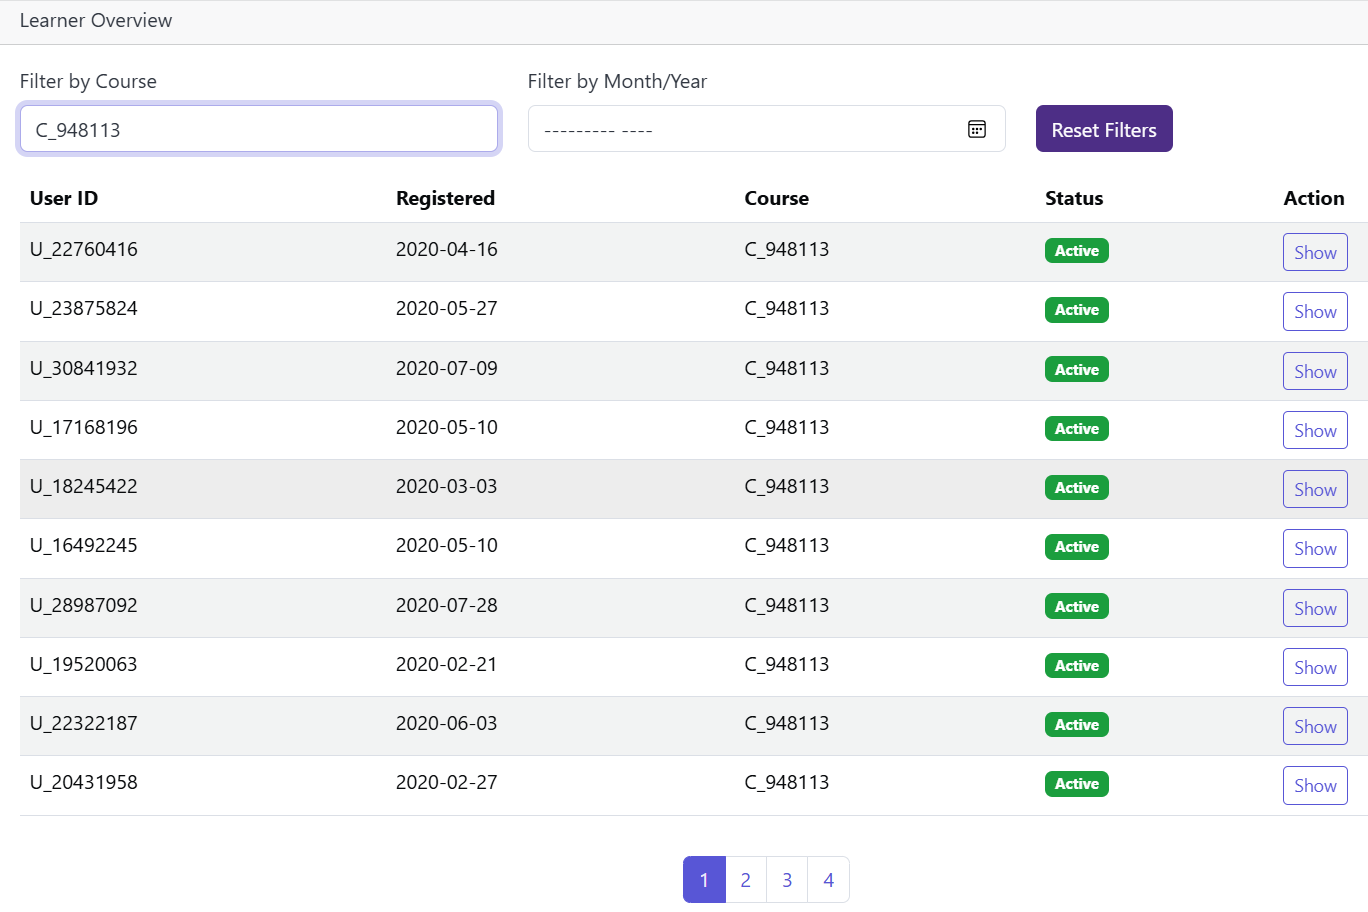
\includegraphics[width = 0.8\textwidth]{imgs/demo-filter.png}
    \caption{Bộ lọc theo khóa học và tháng/năm đăng ký khóa học}
    \label{fig:demo-filter}
\end{figure}
\subsection{Chức năng: Dự đoán kết quả hoàn thành khóa học và xem chi tiết hành vi người học}
\begin{figure}[H]
    \centering
    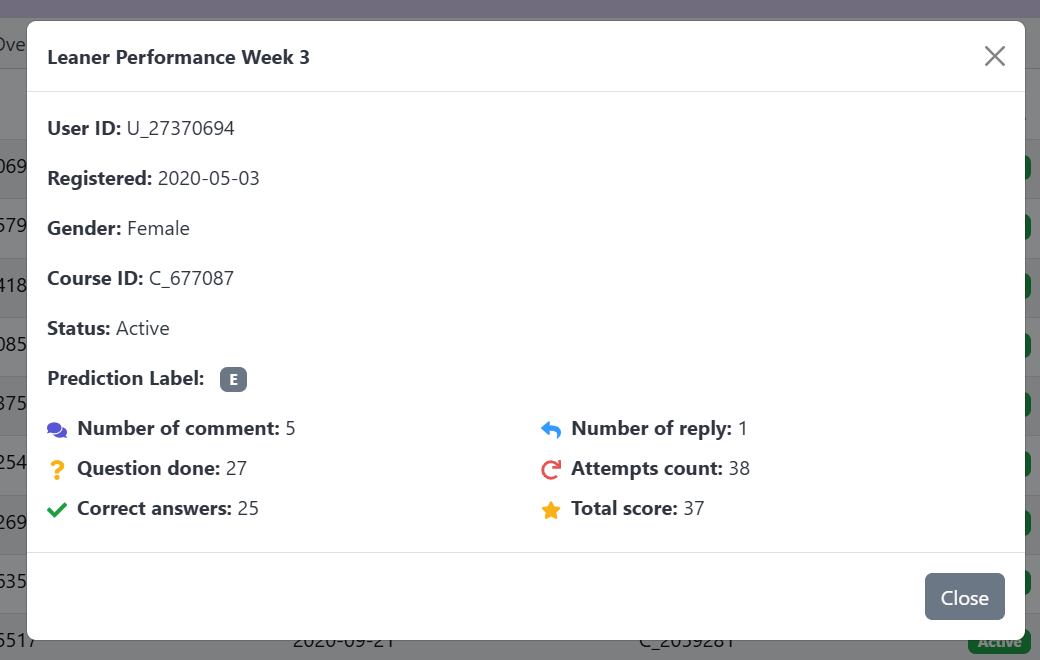
\includegraphics[width = 0.8\textwidth]{imgs/demo-2.png}
    \caption{Dự đoán kết quả hoàn thành khóa học và xem chi tiết hành vi người học}
    \label{fig:demo-2}
\end{figure}
\subsection{Chức năng: Xem xu hướng học tập của người học}
\begin{figure}[H]
    \centering
    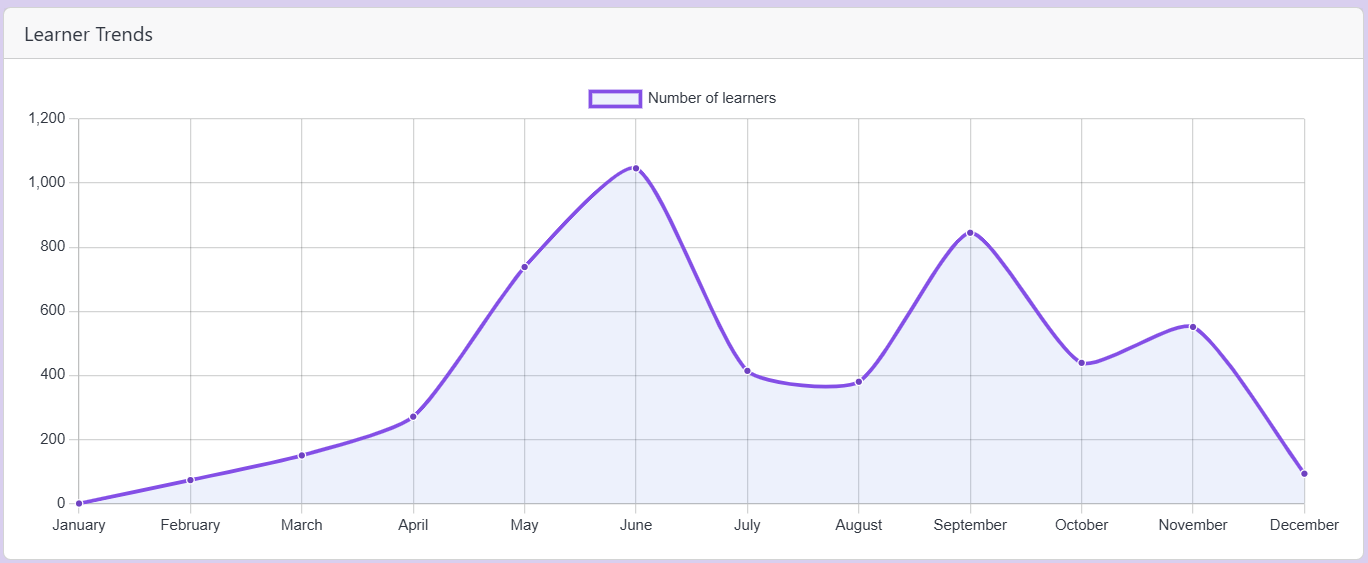
\includegraphics[width = 0.8\textwidth]{imgs/demo-3.png}
    \caption{Xu hướng học tập của người học}
    \label{fig:demo-3}
\end{figure}
\subsection{Chức năng: Xem danh sách 5 khóa học ghi nhận số người học bỏ dở nhiều nhất}
\begin{figure}[H]
    \centering
    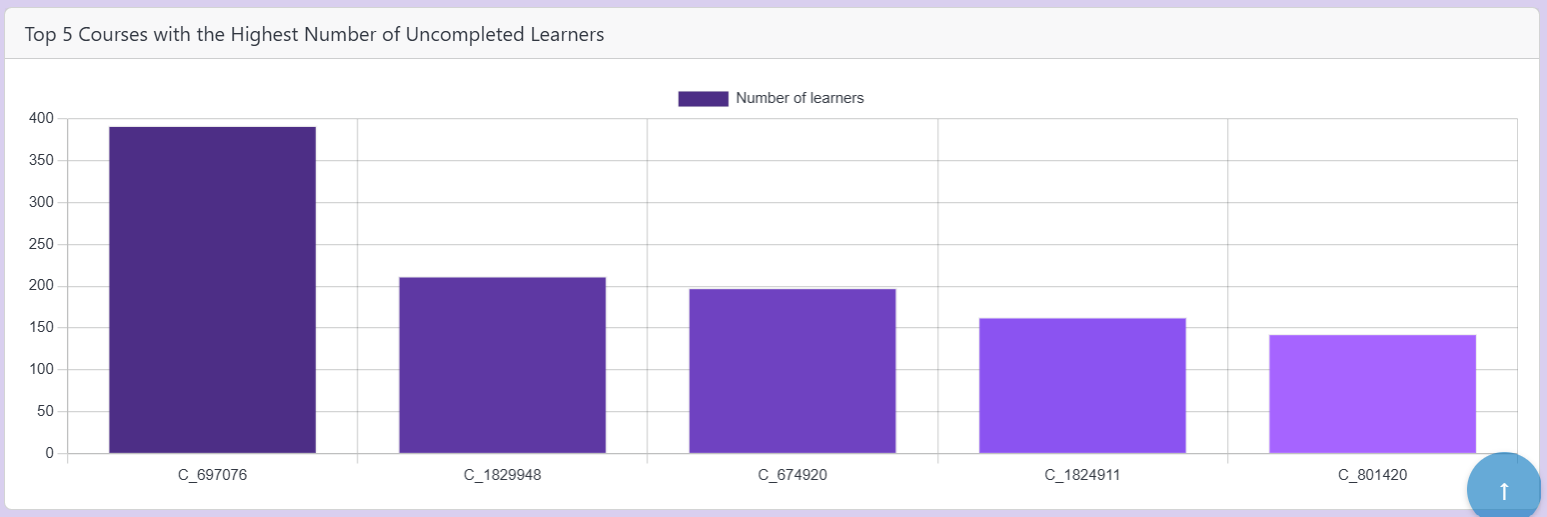
\includegraphics[width = 0.8\textwidth]{imgs/demo-4.png}
    \caption{Danh sách 5 khóa học ghi nhận số người học bỏ dở nhiều nhất}
    \label{fig:demo-4}
\end{figure}
\subsection{Chức năng: Xuất report}
\begin{figure}[H]
    \centering
    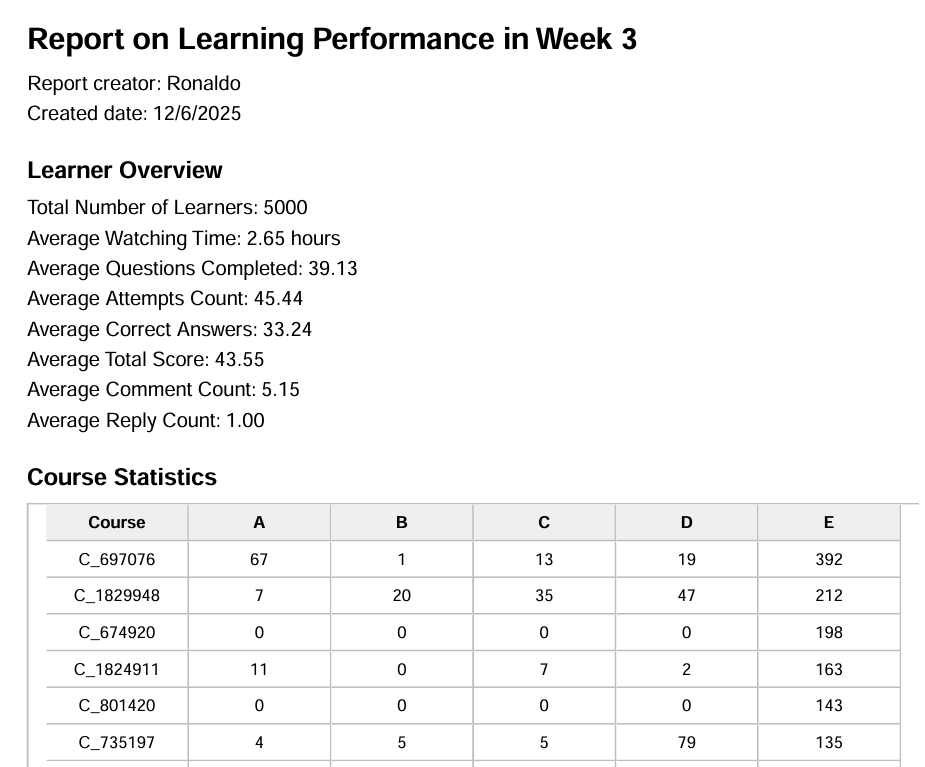
\includegraphics[width = 0.8\textwidth]{imgs/demo-5.png}
    \caption{Mẫu report}
    \label{fig:demo-5}
\end{figure}
\subsection{Chức năng: Xem tổng quát bộ dữ liệu MOOCs}
\begin{figure}[H]
    \centering
    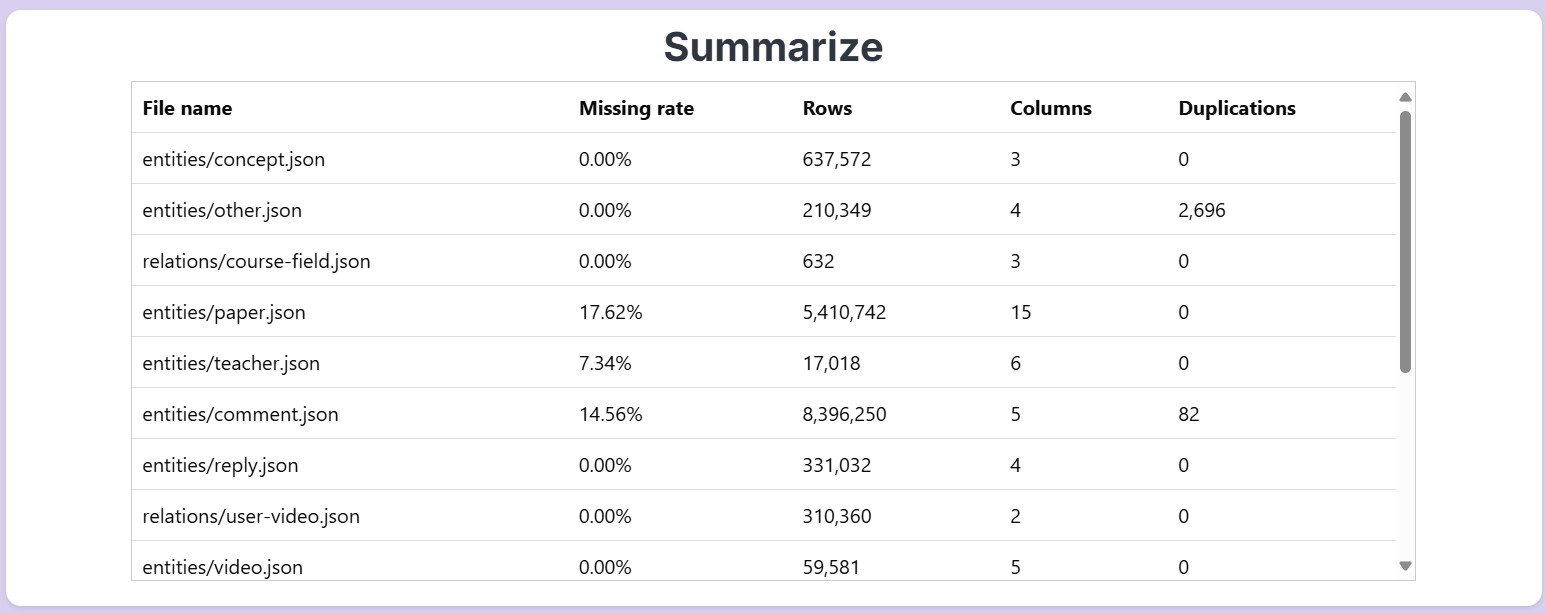
\includegraphics[width = 0.8\textwidth]{imgs/demo-7.png}
    \caption{Tổng quát bộ dữ liệu MOOCs}
    \label{fig:demo-7}
\end{figure}
\subsection{Chức năng: Xem chi tiết từng file dữ liệu MOOCs}
\begin{figure}[H]
    \centering
    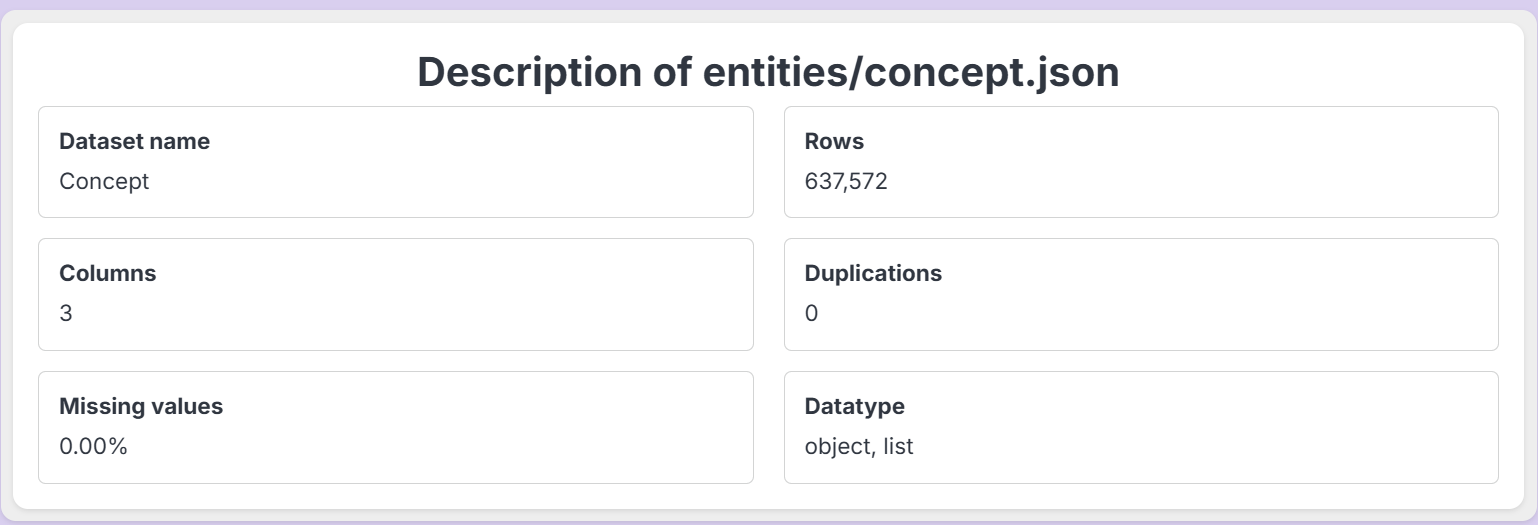
\includegraphics[width = 0.8\textwidth]{imgs/demo-8.png}
    \caption{Chi tiết file dữ liệu concept.json}
    \label{fig:demo-8}
\end{figure}
\subsection{Chức năng: Xem tỷ lệ khuyết của từng file dữ liệu}
\begin{figure}[H]
    \centering
    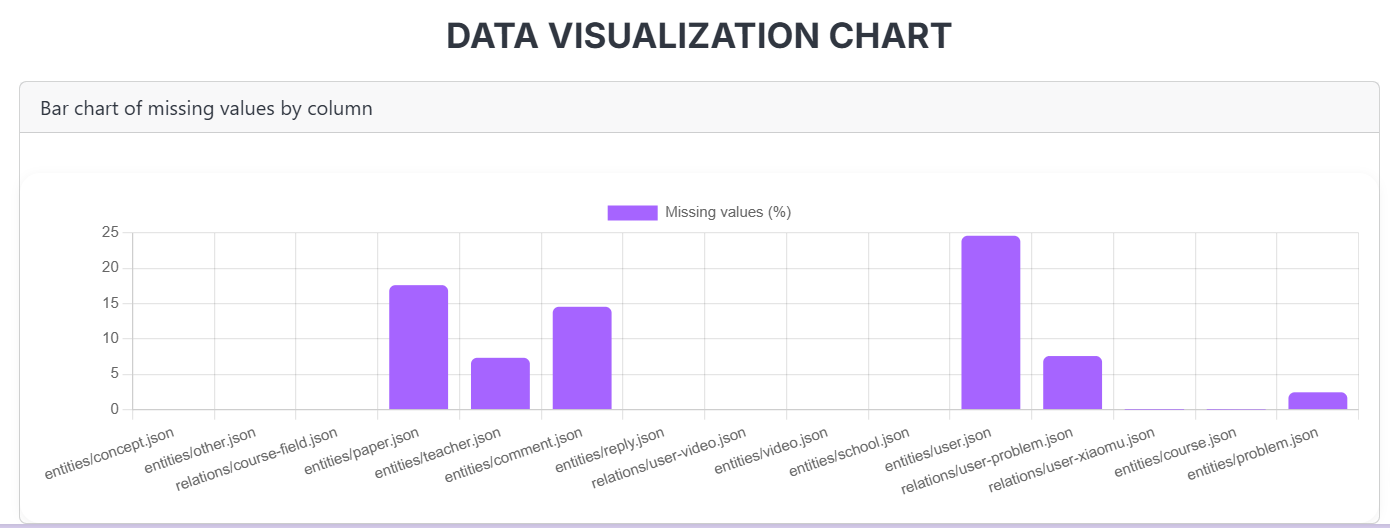
\includegraphics[width = 0.8\textwidth]{imgs/demo-9.png}
    \caption{Biểu đồ tỷ lệ khuyết của từng file dữ liệu}
    \label{fig:demo-9}
\end{figure}
\subsection{Chức năng: Xem chi tiết mô tả bộ dữ liệu hành vi người học}
\begin{figure}[H]
    \centering
    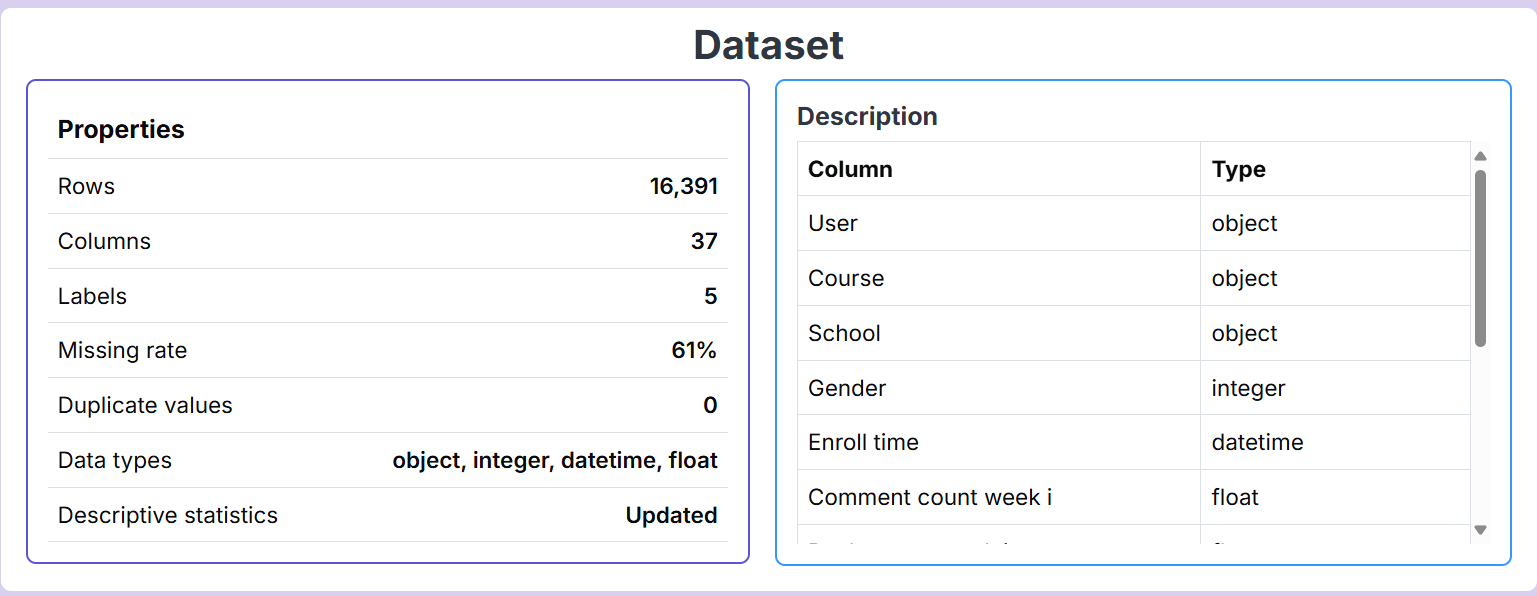
\includegraphics[width = 0.8\textwidth]{imgs/demo-10.png}
    \caption{Mô tả bộ dữ liệu hành vi người học}
    \label{fig:demo-10}
\end{figure}
\subsection{Chức năng: Xem số lượng và tỉ lệ nhãn được dự đoán cho từng người học}
\begin{figure}[H]
    \centering
    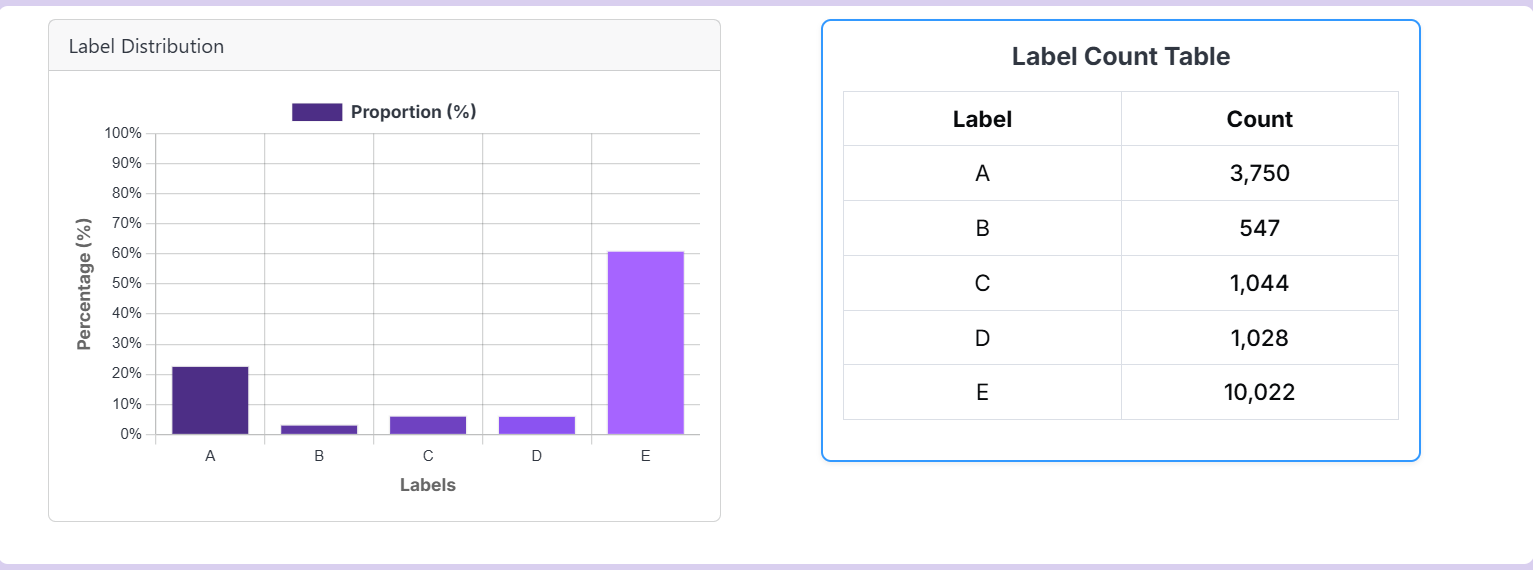
\includegraphics[width = 0.8\textwidth]{imgs/demo-11.png}
    \caption{Biểu đồ tỷ lệ nhãn và bảng số lượng theo từng nhãn}
    \label{fig:demo-11}
\end{figure}
\subsection{Chức năng: Xem chất lượng dữ liệu theo độ đo completeness và consistency}
\begin{figure}[H]
    \centering
    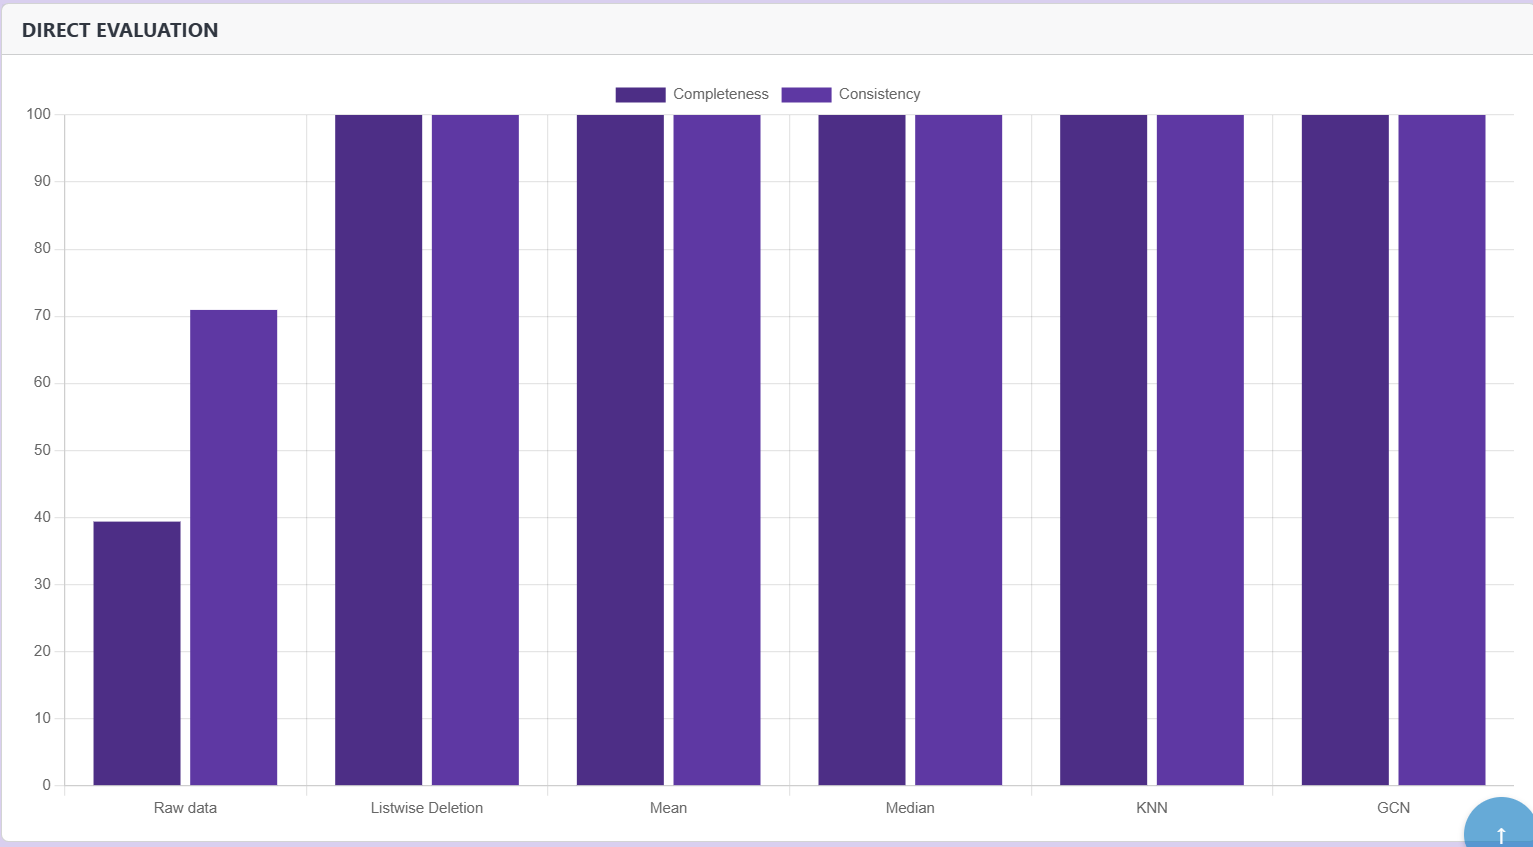
\includegraphics[width = 0.8\textwidth]{imgs/demo-12.png}
    \caption{Biểu đồ chất lượng dữ liệu theo độ đo completeness và consistency}
    \label{fig:demo-12}
\end{figure}
\subsection{Bộ lọc xem hiệu suất dự đoán của từng mô hình}
\begin{figure}[H]
    \centering
    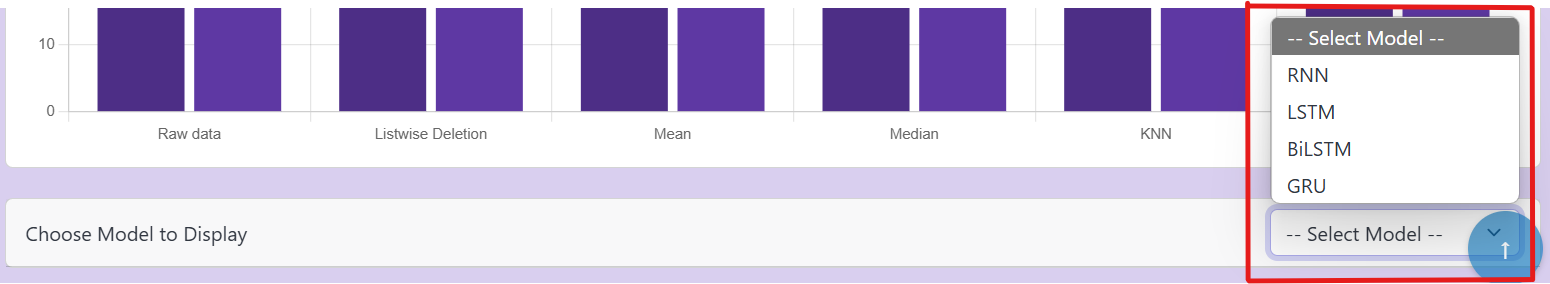
\includegraphics[width = 0.8\textwidth]{imgs/demo-13.png}
    \caption{Bộ lọc kết quả theo mô hình}
    \label{fig:demo-13}
\end{figure}
\begin{figure}[H]
    \centering
    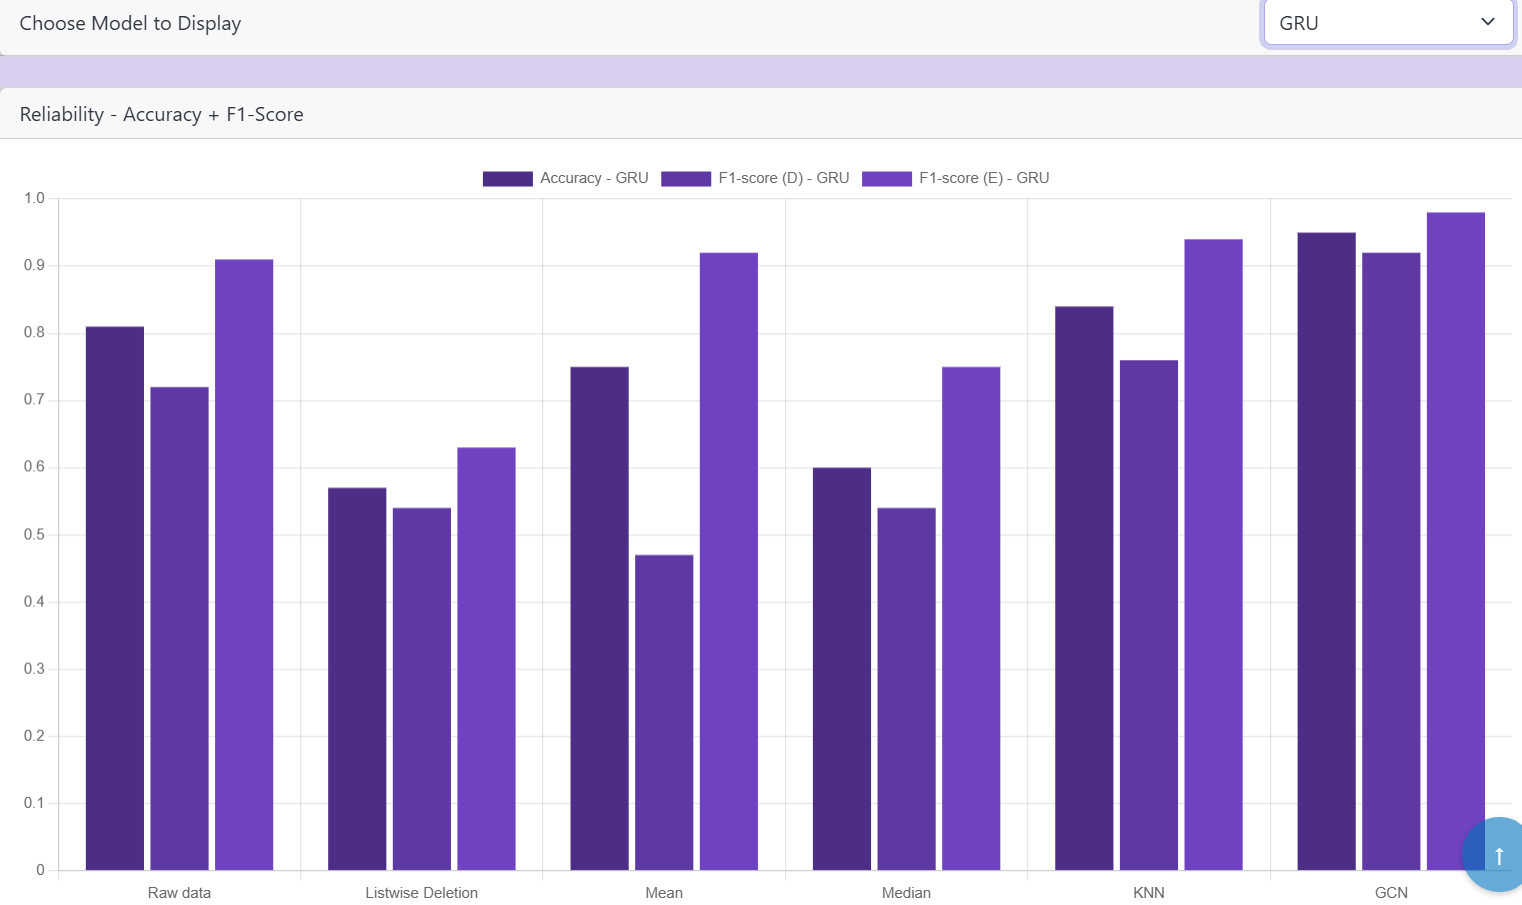
\includegraphics[width = 0.8\textwidth]{imgs/demo-14.png}
    \caption{Accuracy + F1-Score theo mô hình GRU}
    \label{fig:demo-14}
\end{figure}
\begin{figure}[H]
    \centering
    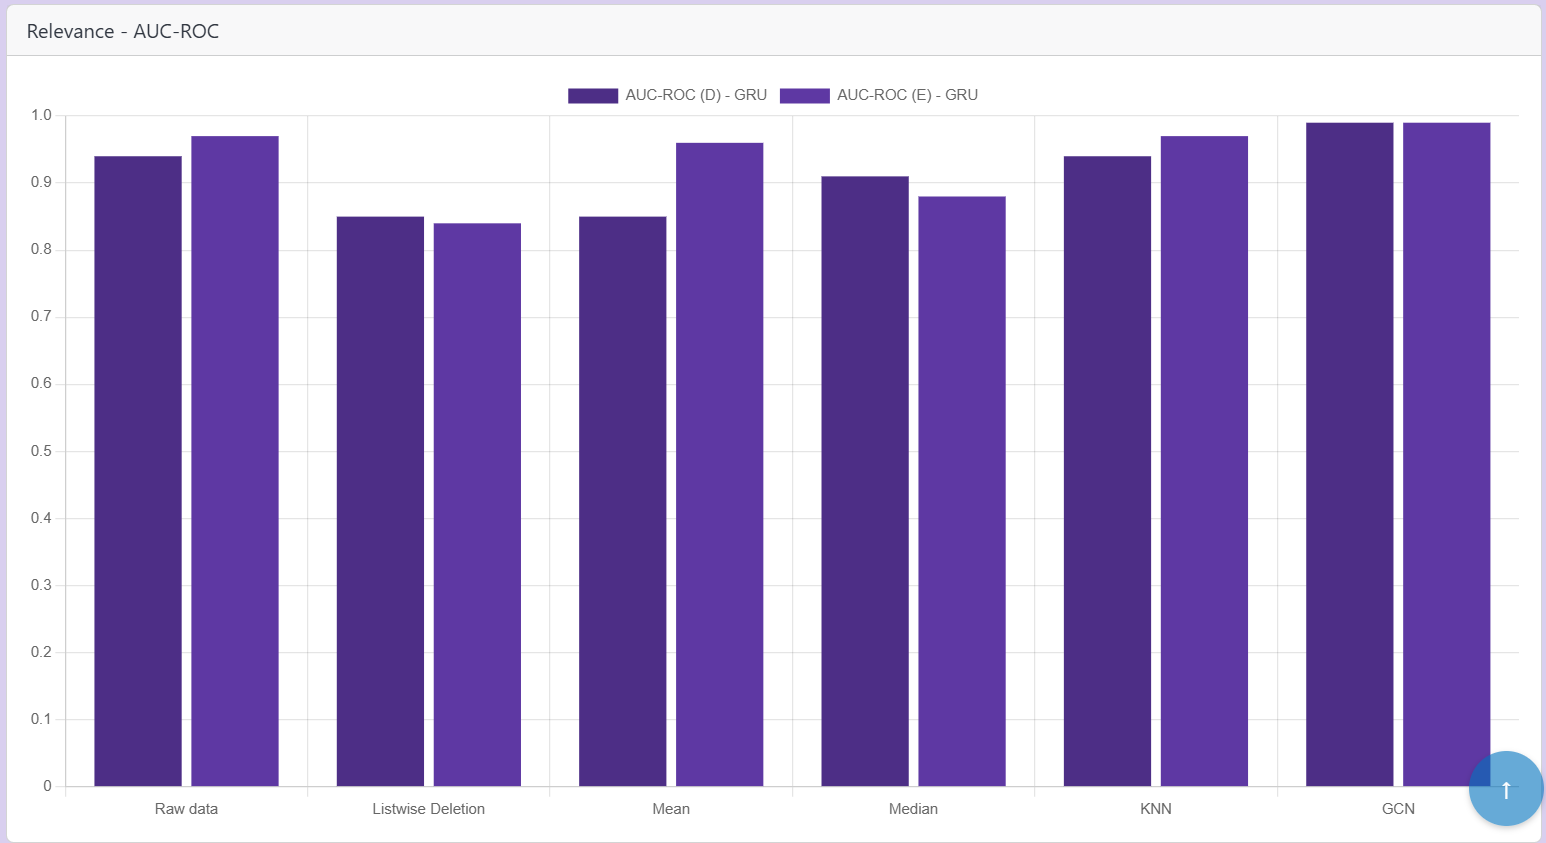
\includegraphics[width = 0.8\textwidth]{imgs/demo-15.png}
    \caption{AUC-ROC theo mô hình GRU}
    \label{fig:demo-15}
\end{figure}
\begin{figure}[H]
    \centering
    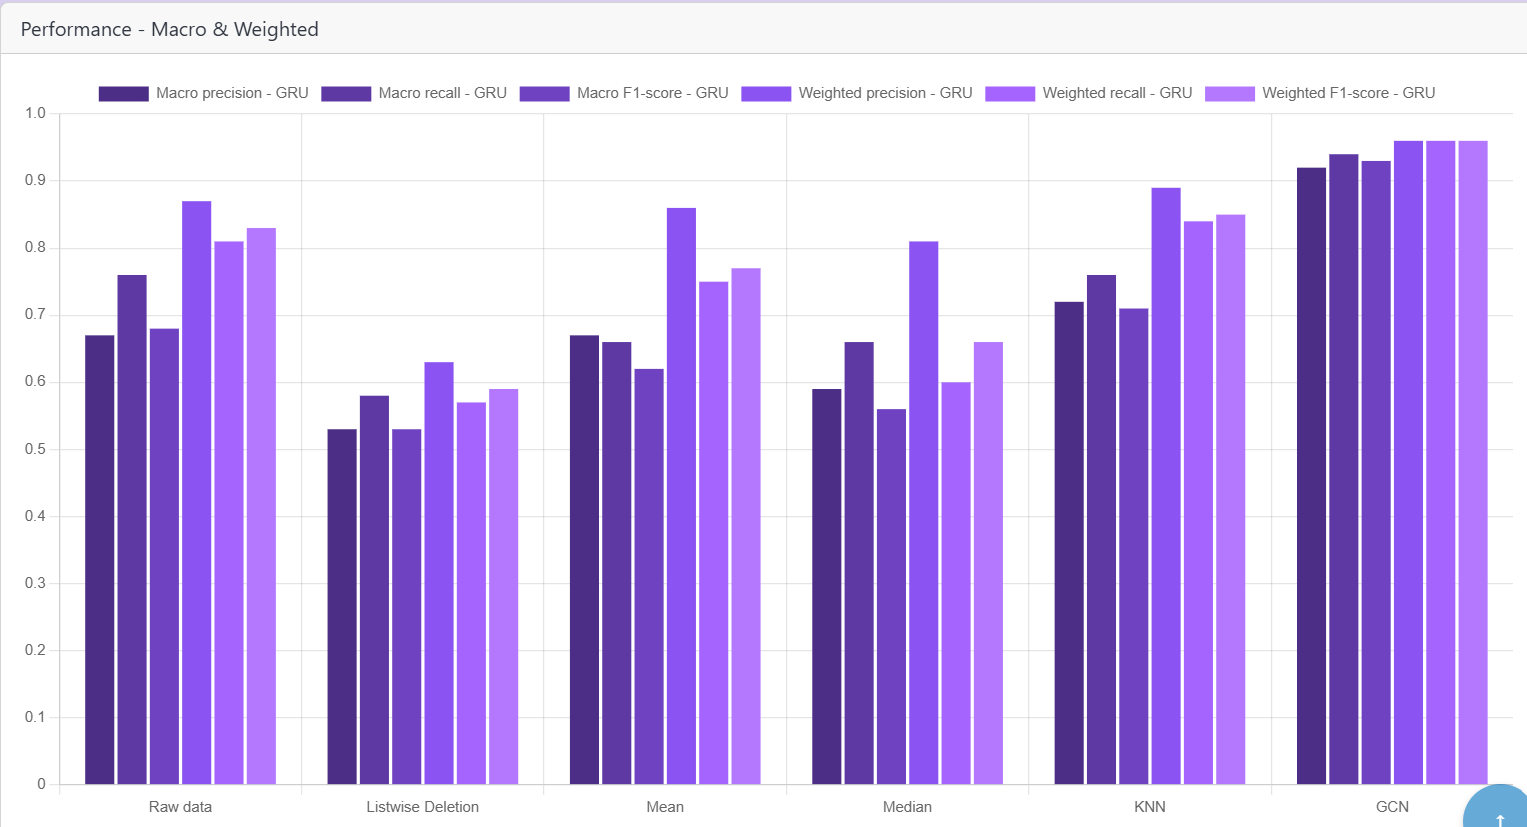
\includegraphics[width = 0.8\textwidth]{imgs/demo-16.png}
    \caption{Hiệu suất toàn diện mô hình GRU theo độ đo Macro và Weighted}
    \label{fig:demo-16}
\end{figure}
